\begin{center}
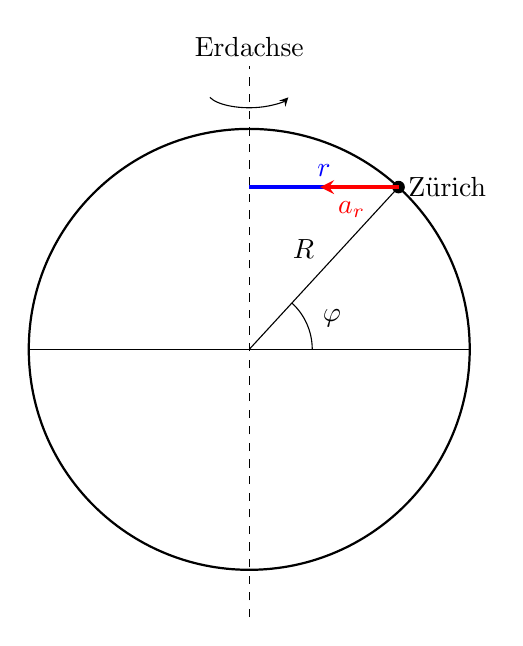
\begin{tikzpicture}[>=stealth]
 \draw[thick] (0,0) circle (2.8);
 \draw[dashed] (0,-3.4) -- (0,3.6) node[above] {Erdachse};
 \draw[->] (-0.5,3.2) arc[start angle=200, end angle=340, x radius=0.53, y radius=0.2];
 \draw (-2.8,0) -- (2.8,0);
 \draw (0,0) -- (1.896,2.061) node[midway, above left] {$R$};
 \draw[very thick, blue] (0,2.061) -- (1.896,2.061) node[midway, above] {$r$};
 \fill (1.896,2.061) circle (0.08) node[right] {Zürich};
 \draw[->, very thick, red] (1.896,2.061) -- (0.9,2.061);
 \node[red, below] at (1.3,2.0) {$a_\text{r}$};
 \draw (0.8,0) arc (0:47.4:0.8);
 \node at (1.05,0.4) {$\varphi$};
\end{tikzpicture}
\end{center}

Zürich (Hönggerberg) liegt auf der geografischen Breite $\varphi = \ang{47;24.6;} = \brO$; die gemessene Fallbeschleunigung ist $g = \gZO$ (FoTaBe S.~204). Der Erdradius ist $R = \rEO$ (FoTaBe S.~212). Zürich bewegt sich in $T = \TeO$ auf einem Kreis um die Erdachse mit dem Radius $r = R\cos\varphi$. Die Radialbeschleunigung ist
\begin{align}
 a_\text{r} &= \frac{4\pi^2 r}{T^2} = \azF \\
   &= \frac{4\pi^2\cdot\rE\cdot\cos\left(\brO\right)}{\left(\Te\right)^2} \\
   &= \az \approx \result{\azP{0}{2}}
\end{align}
Sie zeigt zur Erdachse, nicht zum Erdmittelpunkt. Als Anteil der Fallbeschleunigung:
\begin{align}
 \frac{a_\text{r}}{g} &= \paF = \frac{\az}{\gZ} = \pa \approx \result{\paP{0}{2}}
\end{align}
Rechnet man genauer mit dem Sterntag $T_\text{s} = \TsO$ (FoTaBe S.~205) als Umlaufzeit, erhält man $\pasP{0}{3}$ statt $\paP{0}{3}$; auf zwei Stellen ändert sich nichts.
